% TikZ diagrams for competition technical document
% Compile: pdflatex -interaction=nonstopmode tikz_diagrams.tex
\documentclass[tikz,border=3pt]{standalone}

\usepackage{tikz}
\usepackage{amsmath}
\usepackage{amssymb}
\usepackage{mathpazo}
\usepackage[T1]{fontenc}

\usetikzlibrary{
  positioning,
  shapes.geometric,
  shapes.multipart,
  arrows.meta,
  fit,
  backgrounds,
  calc,
  decorations.pathreplacing,
  matrix,
  patterns,
  shadows.blur,
}

% ── Color palette (academic grayscale) ──
\definecolor{bg}{HTML}{FFFFFF}
\definecolor{border}{HTML}{333333}
\definecolor{fillMain}{HTML}{F5F5F5}
\definecolor{fillAcc}{HTML}{EBEBEB}
\definecolor{fillDark}{HTML}{DDDDDD}
\definecolor{textCol}{HTML}{222222}
\definecolor{textSub}{HTML}{666666}
\definecolor{arrowCol}{HTML}{555555}
\definecolor{layerGray}{HTML}{999999}

% ── Styles ──
\tikzset{
  mainbox/.style={
    rectangle, rounded corners=2pt, draw=border, fill=fillMain,
    minimum width=2.2cm, minimum height=0.8cm, align=center,
    font=\footnotesize, inner sep=4pt, line width=0.5pt,
  },
  darkbox/.style={
    mainbox, fill=fillDark, font=\footnotesize\bfseries,
  },
  accentbox/.style={
    mainbox, fill=fillAcc, draw=border!80, line width=0.7pt,
  },
  dashframe/.style={
    rectangle, rounded corners=1pt, draw=layerGray, dashed,
    inner sep=2pt, line width=0.4pt,
  },
  arrow/.style={-{Stealth[scale=0.7]}, arrowCol, line width=0.5pt},
  darrow/.style={-{Stealth[scale=0.6]}, arrowCol!60, line width=0.4pt, dashed},
  label/.style={font=\footnotesize\bfseries, text=textSub},
}

% ═══════════════════════════════════════════════════════════════
\begin{document}

% ── FIGURE 1: System Architecture ──
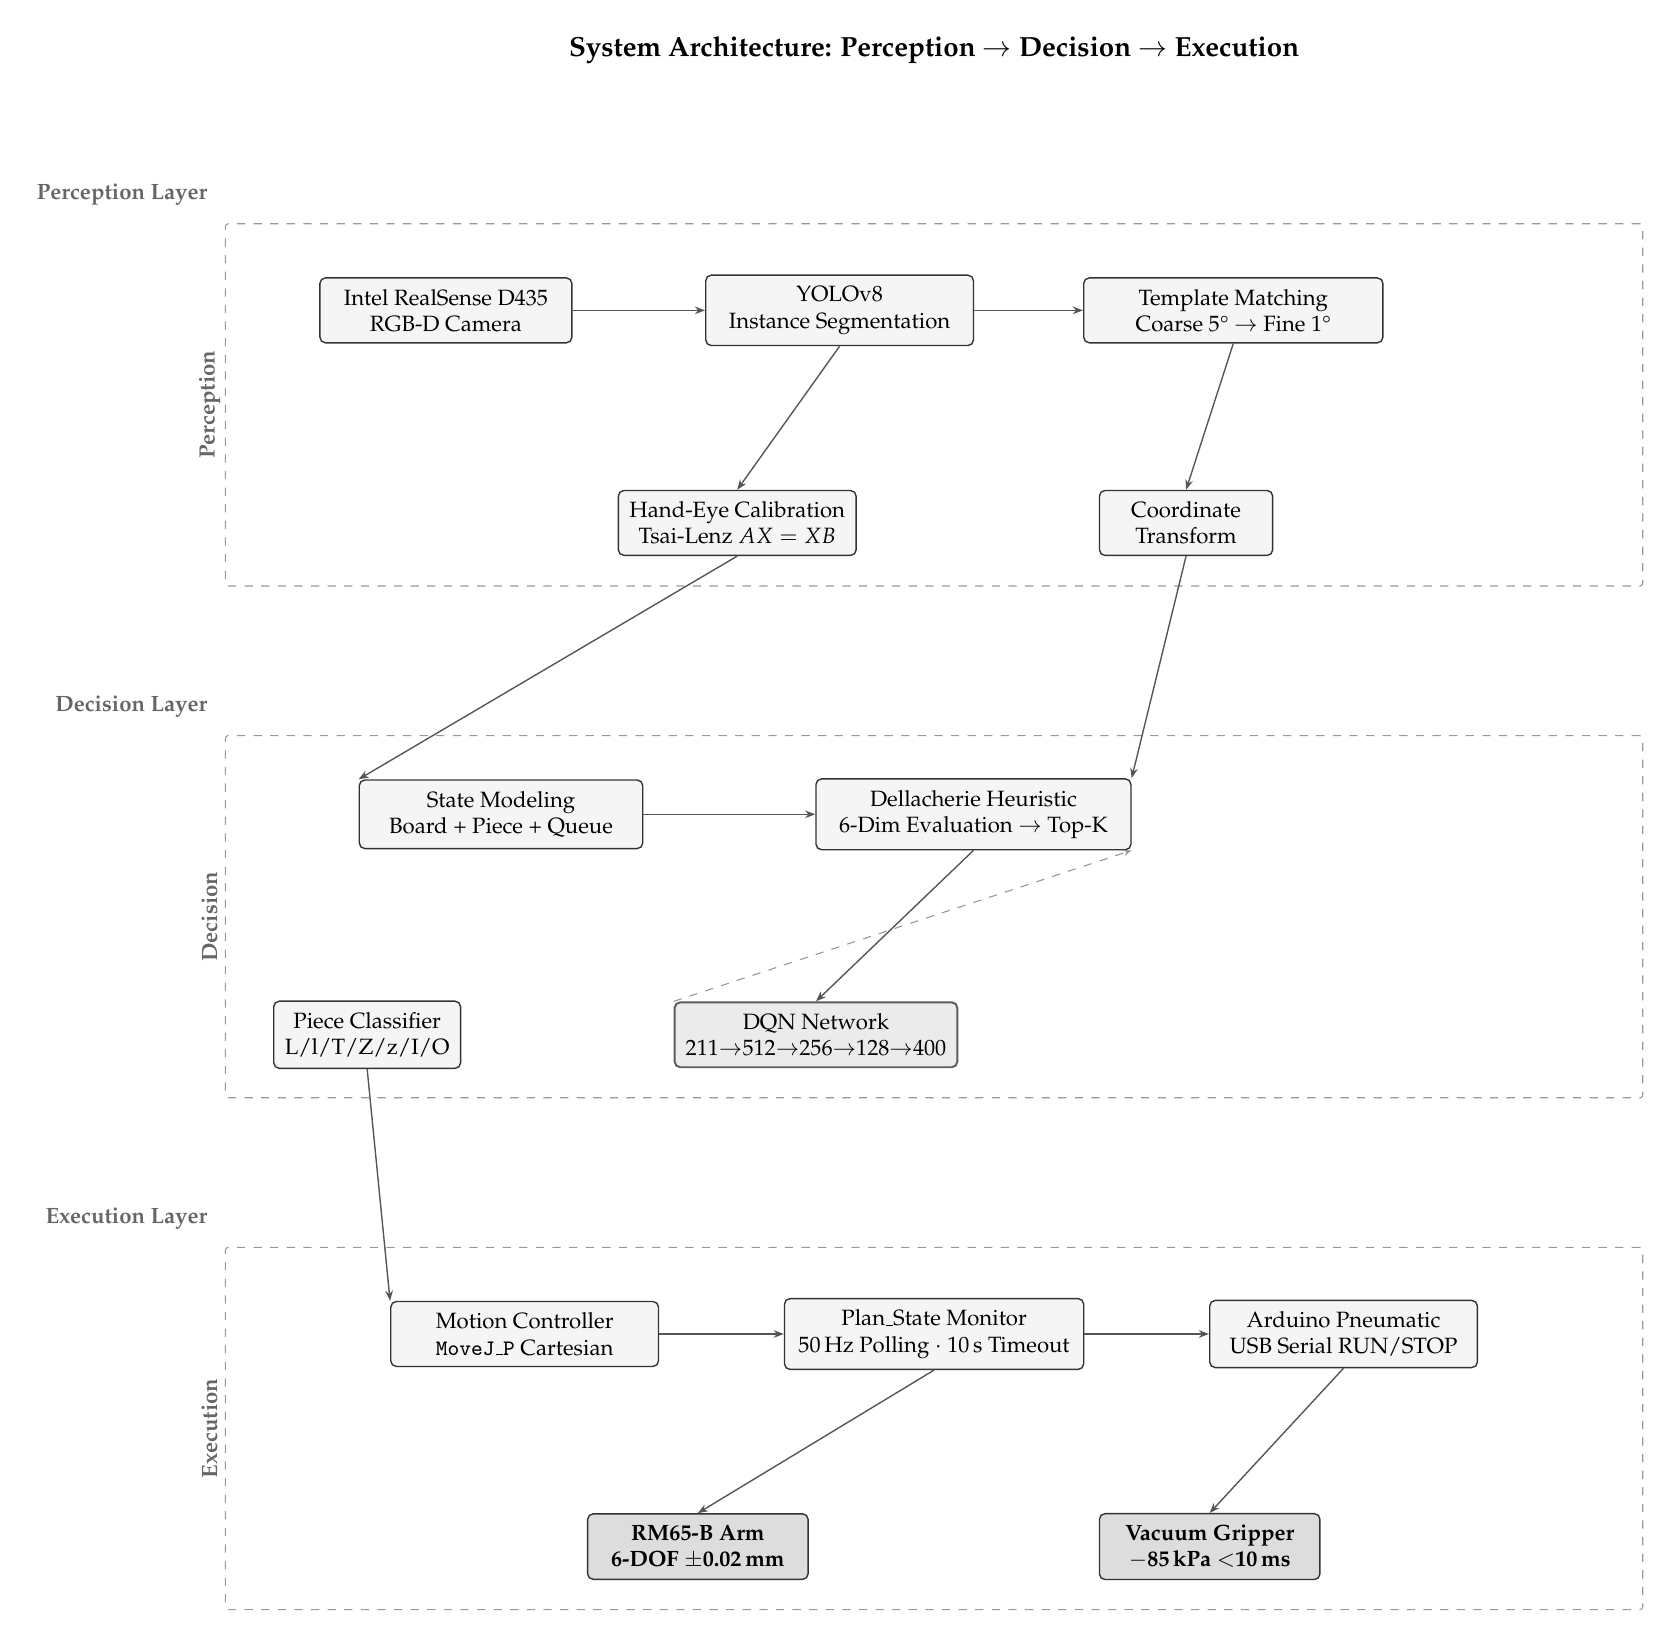
\begin{tikzpicture}[node distance=0.6cm]

  \node[label, rotate=90] at (-9.2, 7) {Perception};
  \node[label, rotate=90] at (-9.2, 0.5) {Decision};
  \node[label, rotate=90] at (-9.2, -6) {Execution};

  % Perception layer
  \node[dashframe, minimum width=18cm, minimum height=4.6cm] (Pframe) at (0, 7) {};
  \node[label, above left=1mm and 1mm of Pframe.north west] {\footnotesize Perception Layer};

  \node[mainbox, minimum width=3.2cm] (cam) at (-6.2, 8.2) {Intel RealSense D435\\RGB-D Camera};
  \node[mainbox, minimum width=3.4cm] (yolo) at (-1.2, 8.2) {YOLOv8\\Instance Segmentation};
  \node[mainbox, minimum width=3.8cm] (tm) at (3.8, 8.2) {Template Matching\\Coarse 5\textdegree{} $\rightarrow$ Fine 1\textdegree{}};
  \node[mainbox, minimum width=2.6cm] (he) at (-2.5, 5.5) {Hand-Eye Calibration\\Tsai-Lenz $AX=XB$};
  \node[mainbox, minimum width=2.2cm] (tf) at (3.2, 5.5) {Coordinate\\Transform};

  \draw[arrow] (cam) -- (yolo);
  \draw[arrow] (yolo) -- (tm);
  \draw[arrow] (yolo.south) -- (he.north);
  \draw[arrow] (tm.south) -- (tf.north);

  % Decision layer
  \node[dashframe, minimum width=18cm, minimum height=4.6cm] (Dframe) at (0, 0.5) {};
  \node[label, above left=1mm and 1mm of Dframe.north west] {\footnotesize Decision Layer};

  \node[mainbox, minimum width=3.6cm] (state) at (-5.5, 1.8) {State Modeling\\Board + Piece + Queue};
  \node[mainbox, minimum width=4cm] (heur) at (0.5, 1.8) {Dellacherie Heuristic\\6-Dim Evaluation $\rightarrow$ Top-K};
  \node[accentbox, minimum width=3.4cm] (dqn) at (-1.5, -1) {DQN Network\\211$\rightarrow$512$\rightarrow$256$\rightarrow$128$\rightarrow$400};
  \node[mainbox, minimum width=2.2cm] (cls) at (-7.2, -1) {Piece Classifier\\L/l/T/Z/z/I/O};

  \draw[arrow] (state) -- (heur);
  \draw[arrow] (heur.south) -- (dqn.north);
  \draw[darrow] (dqn.north west) -- (heur.south east);

  % Execution layer
  \node[dashframe, minimum width=18cm, minimum height=4.6cm] (Eframe) at (0, -6) {};
  \node[label, above left=1mm and 1mm of Eframe.north west] {\footnotesize Execution Layer};

  \node[mainbox, minimum width=3.4cm] (mot) at (-5.2, -4.8) {Motion Controller\\\texttt{MoveJ\_P} Cartesian};
  \node[mainbox, minimum width=3.8cm] (mon) at (0, -4.8) {Plan\_State Monitor\\50\,Hz Polling $\cdot$ 10\,s Timeout};
  \node[mainbox, minimum width=3.4cm] (ard) at (5.2, -4.8) {Arduino Pneumatic\\USB Serial RUN/STOP};
  \node[darkbox, minimum width=2.8cm] (arm) at (-3, -7.5) {RM65-B Arm\\6-DOF $\pm$0.02\,mm};
  \node[darkbox, minimum width=2.8cm] (vac) at (3.5, -7.5) {Vacuum Gripper\\$-$85\,kPa $<$10\,ms};

  \draw[arrow] (mot) -- (mon);
  \draw[arrow] (mon) -- (ard);
  \draw[arrow] (mon.south) -- (arm.north);
  \draw[arrow] (ard.south) -- (vac.north);

  % Inter-layer
  \draw[arrow] (he.south) -- (state.north west);
  \draw[arrow] (tf.south) -- (heur.north east);
  \draw[arrow] (cls.south) -- (mot.north west);

  % Title
  \node[font=\normalsize\bfseries] at (0, 11.5) {System Architecture: Perception $\rightarrow$ Decision $\rightarrow$ Execution};

\end{tikzpicture}

% ── FIGURE 2: ROS Node Communication Graph ──
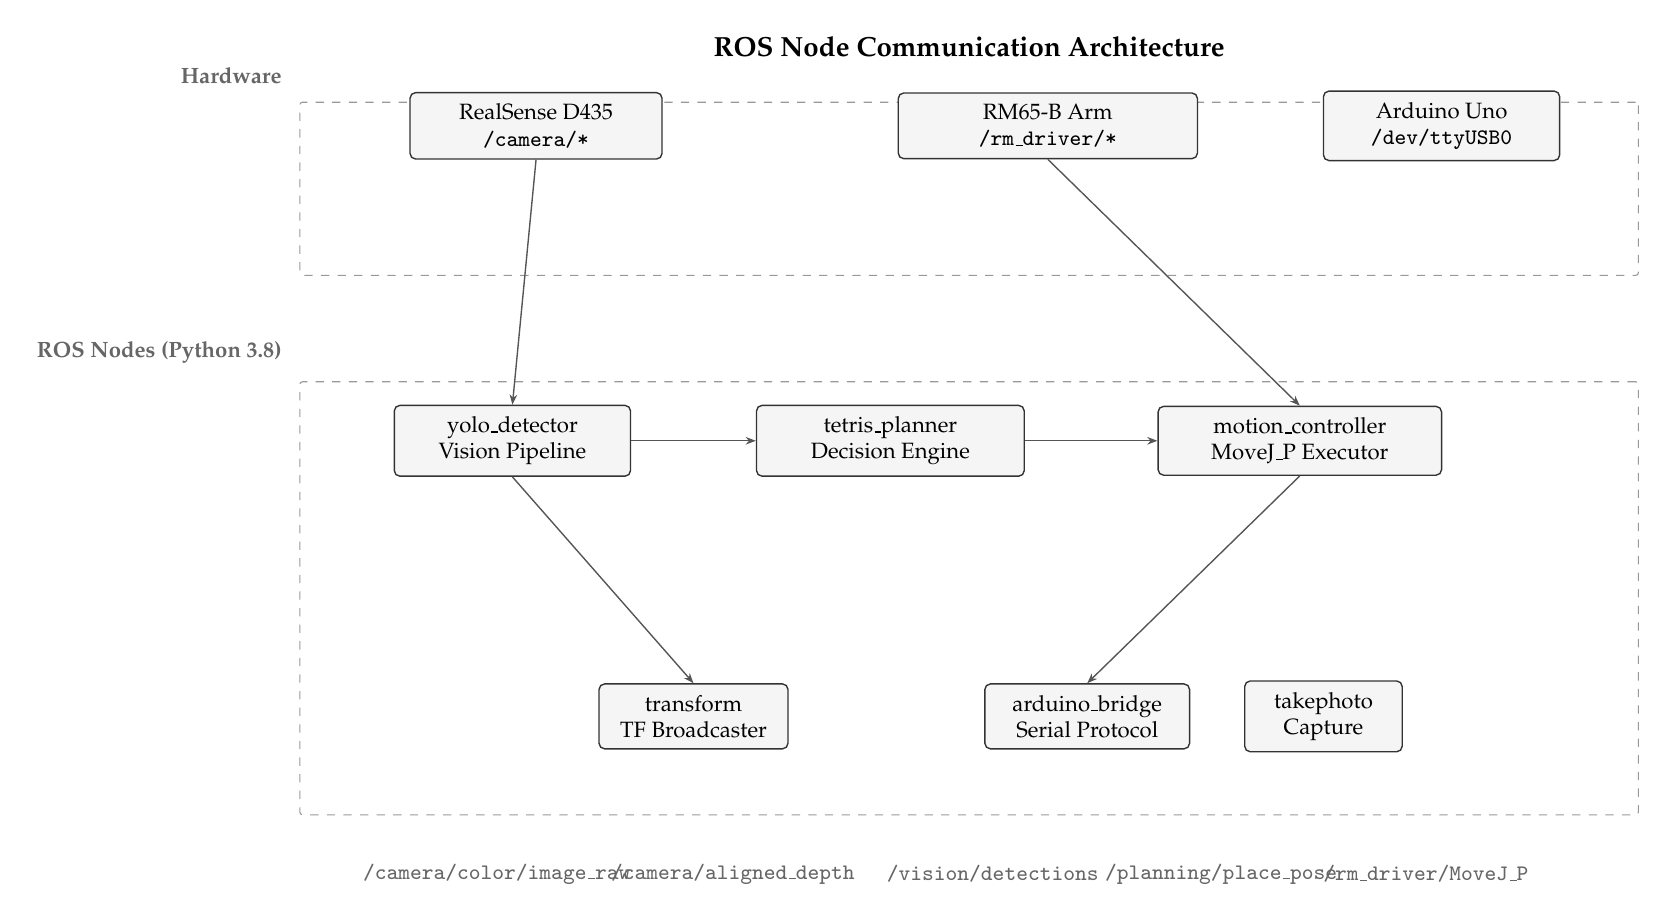
\begin{tikzpicture}[node distance=0.5cm]

  \node[font=\normalsize\bfseries] at (0, 9) {ROS Node Communication Architecture};

  % Hardware
  \node[dashframe, minimum width=17cm, minimum height=2.2cm] (hwframe) at (0, 7.2) {};
  \node[label, above left=1mm and 1mm of hwframe.north west] {\footnotesize Hardware};
  \node[mainbox, minimum width=3.2cm] (dcam) at (-5.5, 8) {RealSense D435\\\texttt{/camera/*}};
  \node[mainbox, minimum width=3.8cm] (darm) at (1, 8) {RM65-B Arm\\\texttt{/rm\_driver/*}};
  \node[mainbox, minimum width=3cm] (duno) at (6, 8) {Arduino Uno\\\texttt{/dev/ttyUSB0}};

  % ROS Nodes
  \node[dashframe, minimum width=17cm, minimum height=5.5cm] (rosframe) at (0, 2) {};
  \node[label, above left=1mm and 1mm of rosframe.north west] {\footnotesize ROS Nodes (Python 3.8)};

  \node[mainbox, minimum width=3cm] (nyolo) at (-5.8, 4) {yolo\_detector\\Vision Pipeline};
  \node[mainbox, minimum width=3.4cm] (nplan) at (-1, 4) {tetris\_planner\\Decision Engine};
  \node[mainbox, minimum width=3.6cm] (nmot) at (4.2, 4) {motion\_controller\\MoveJ\_P Executor};
  \node[mainbox, minimum width=2.4cm] (ntf) at (-3.5, 0.5) {transform\\TF Broadcaster};
  \node[mainbox, minimum width=2.6cm] (nser) at (1.5, 0.5) {arduino\_bridge\\Serial Protocol};
  \node[mainbox, minimum width=2cm] (ncap) at (4.5, 0.5) {takephoto\\Capture};

  \draw[arrow] (nyolo) -- (nplan);
  \draw[arrow] (nplan) -- (nmot);
  \draw[arrow] (nyolo.south) -- (ntf.north);
  \draw[arrow] (nmot.south) -- (nser.north);

  % Topics
  \node[font=\footnotesize, text=textSub] at (-6, -1.5) {\texttt{/camera/color/image\_raw}};
  \node[font=\footnotesize, text=textSub] at (-3, -1.5) {\texttt{/camera/aligned\_depth}};
  \node[font=\footnotesize, text=textSub] at (0.3, -1.5) {\texttt{/vision/detections}};
  \node[font=\footnotesize, text=textSub] at (3.2, -1.5) {\texttt{/planning/place\_pose}};
  \node[font=\footnotesize, text=textSub] at (5.8, -1.5) {\texttt{/rm\_driver/MoveJ\_P}};

  \draw[arrow] (dcam.south) -- (nyolo.north);
  \draw[arrow] (darm.south) -- (nmot.north);

\end{tikzpicture}

% ── FIGURE 3: Vision Pipeline ──
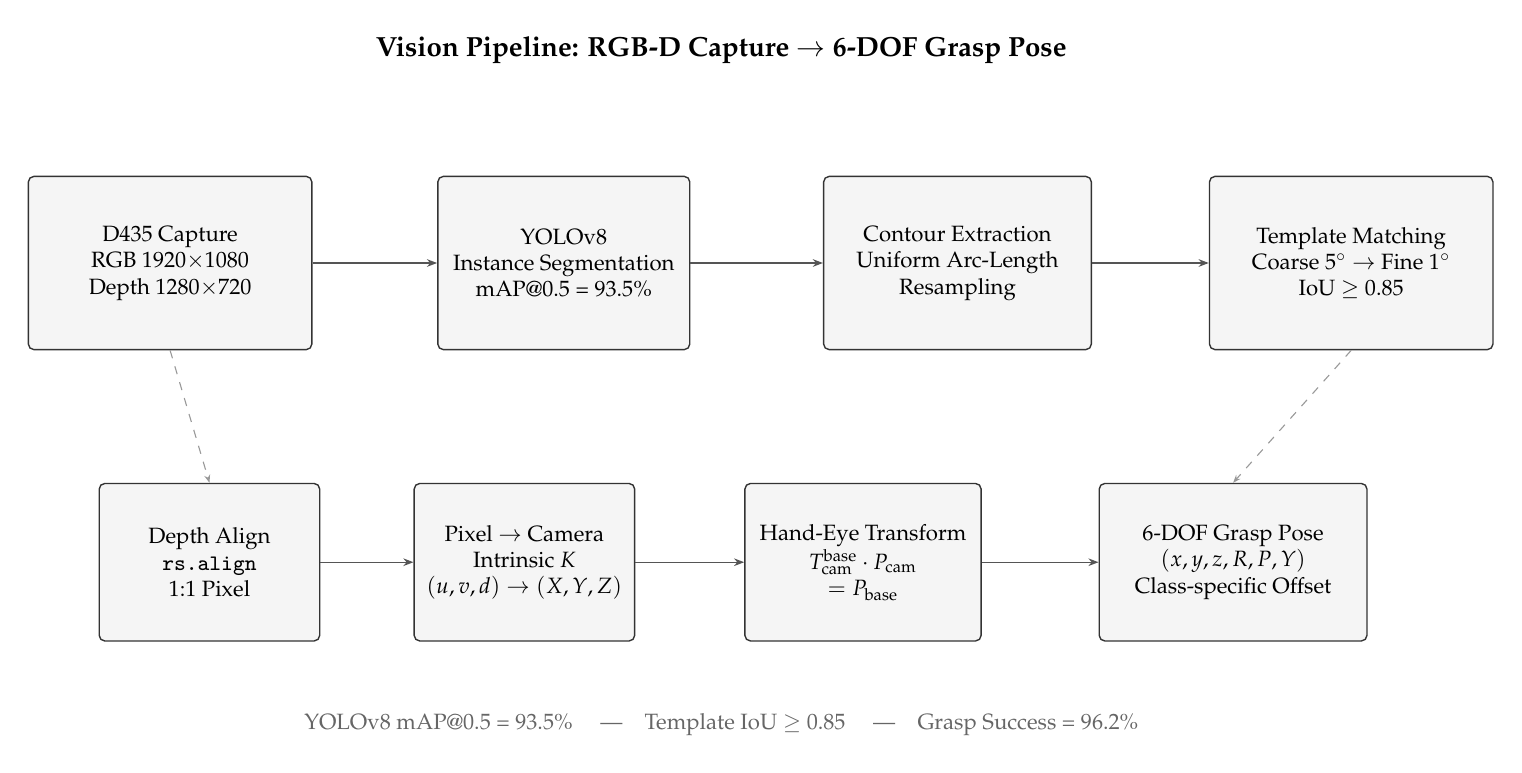
\begin{tikzpicture}[node distance=0.5cm]

  \node[font=\normalsize\bfseries] at (0, 6.5) {Vision Pipeline: RGB-D Capture $\rightarrow$ 6-DOF Grasp Pose};

  % Top row
  \node[mainbox, minimum width=3.6cm, minimum height=2.2cm] (v1) at (-7, 3.8) {D435 Capture\\RGB 1920$\times$1080\\Depth 1280$\times$720};
  \node[mainbox, minimum width=3.2cm, minimum height=2.2cm] (v2) at (-2, 3.8) {YOLOv8\\Instance Segmentation\\mAP@0.5 = 93.5\%};
  \node[mainbox, minimum width=3.4cm, minimum height=2.2cm] (v3) at (3, 3.8) {Contour Extraction\\Uniform Arc-Length\\Resampling};
  \node[mainbox, minimum width=3.6cm, minimum height=2.2cm] (v4) at (8, 3.8) {Template Matching\\Coarse $5^\circ$ $\rightarrow$ Fine $1^\circ$\\IoU $\geq$ 0.85};

  % Bottom row
  \node[mainbox, minimum width=2.8cm, minimum height=2cm] (v5) at (-6.5, 0) {Depth Align\\\texttt{rs.align}\\1:1 Pixel};
  \node[mainbox, minimum width=2.8cm, minimum height=2cm] (v6) at (-2.5, 0) {Pixel $\rightarrow$ Camera\\Intrinsic $K$\\$(u,v,d)\rightarrow(X,Y,Z)$};
  \node[mainbox, minimum width=3cm, minimum height=2cm] (v7) at (1.8, 0) {Hand-Eye Transform\\$T_\text{cam}^\text{base}\cdot P_\text{cam}$\\$= P_\text{base}$};
  \node[mainbox, minimum width=3.4cm, minimum height=2cm] (v8) at (6.5, 0) {6-DOF Grasp Pose\\$(x,y,z,R,P,Y)$\\Class-specific Offset};

  \draw[arrow] (v1) -- (v2);
  \draw[arrow] (v2) -- (v3);
  \draw[arrow] (v3) -- (v4);
  \draw[arrow] (v5) -- (v6);
  \draw[arrow] (v6) -- (v7);
  \draw[arrow] (v7) -- (v8);

  \draw[darrow] (v1.south) -- (v5.north);
  \draw[darrow] (v4.south) -- (v8.north);

  \node[font=\footnotesize, text=textSub, below=0.8cm] at (0, -1.0) {YOLOv8 mAP@0.5 = 93.5\% \quad|\quad Template IoU $\geq$ 0.85 \quad|\quad Grasp Success = 96.2\%};

\end{tikzpicture}

% ── FIGURE 4: Hybrid Decision Flow ──
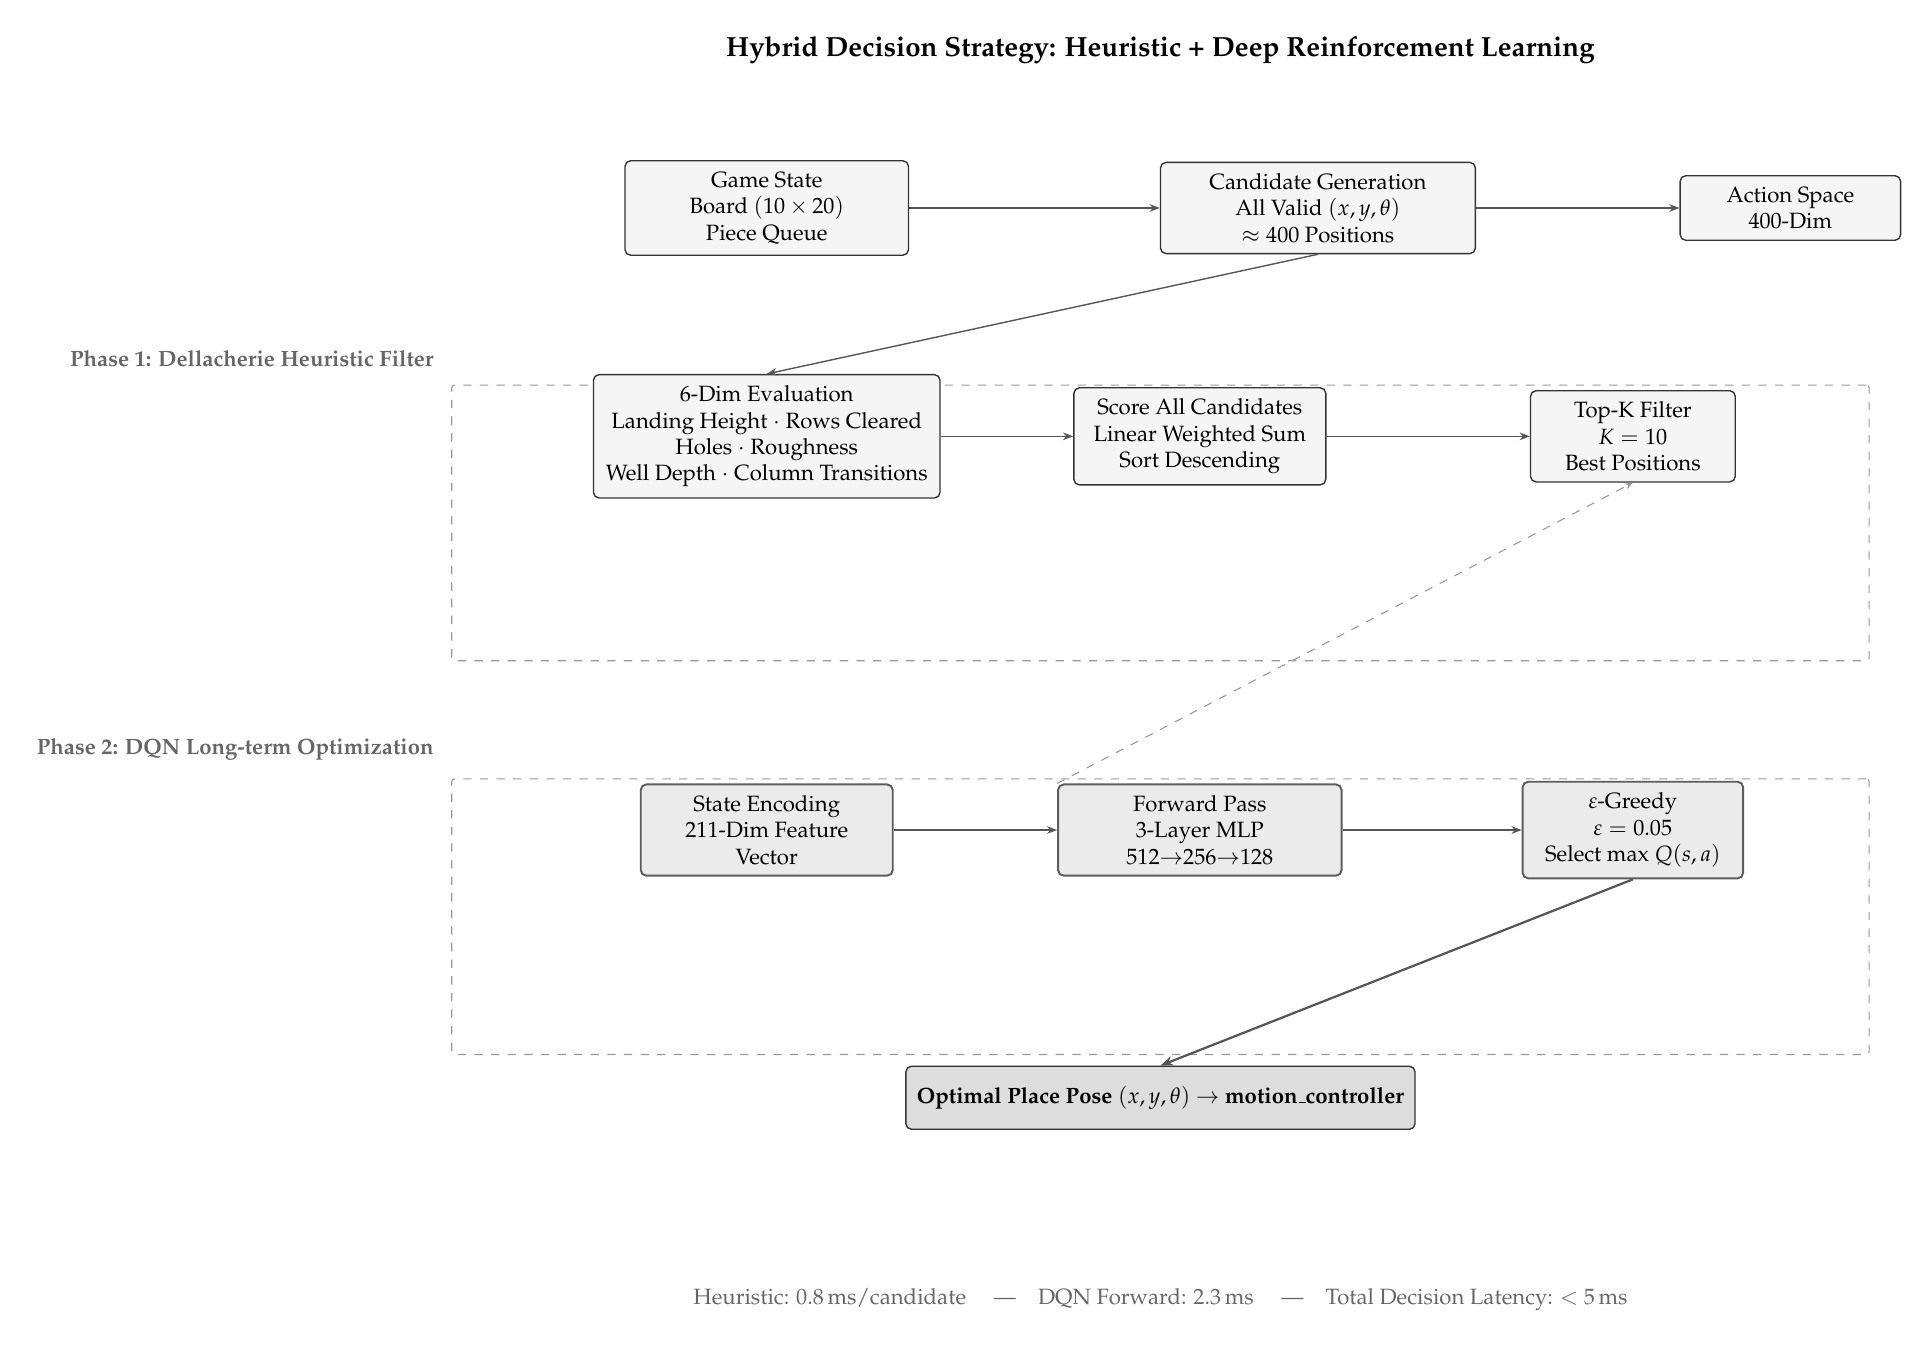
\begin{tikzpicture}[node distance=0.5cm]

  \node[font=\normalsize\bfseries] at (0, 9.5) {Hybrid Decision Strategy: Heuristic + Deep Reinforcement Learning};

  % Inputs
  \node[mainbox, minimum width=3.6cm] (inp) at (-5, 7.5) {Game State\\Board $(10\times 20)$\\Piece Queue};
  \node[mainbox, minimum width=4cm] (cand) at (2, 7.5) {Candidate Generation\\All Valid $(x,y,\theta)$\\$\approx 400$ Positions};
  \node[mainbox, minimum width=2.8cm] (act) at (8, 7.5) {Action Space\\400-Dim};
  \draw[arrow] (inp) -- (cand);
  \draw[arrow] (cand) -- (act);

  % Phase 1
  \node[dashframe, minimum width=18cm, minimum height=3.5cm] (p1frame) at (0, 3.5) {};
  \node[label, above left=1mm and 1mm of p1frame.north west] {\footnotesize Phase 1: Dellacherie Heuristic Filter};

  \node[mainbox, minimum width=4.4cm] (feat) at (-5, 4.6) {6-Dim Evaluation\\Landing Height $\cdot$ Rows Cleared\\Holes $\cdot$ Roughness\\Well Depth $\cdot$ Column Transitions};
  \node[mainbox, minimum width=3.2cm] (score) at (0.5, 4.6) {Score All Candidates\\Linear Weighted Sum\\Sort Descending};
  \node[mainbox, minimum width=2.6cm] (topk) at (6, 4.6) {Top-K Filter\\$K=10$\\Best Positions};

  \draw[arrow] (feat) -- (score);
  \draw[arrow] (score) -- (topk);
  \draw[arrow] (cand.south) -- (feat.north);

  % Phase 2
  \node[dashframe, minimum width=18cm, minimum height=3.5cm] (p2frame) at (0, -1.5) {};
  \node[label, above left=1mm and 1mm of p2frame.north west] {\footnotesize Phase 2: DQN Long-term Optimization};

  \node[accentbox, minimum width=3.2cm] (enc) at (-5, -0.4) {State Encoding\\211-Dim Feature\\Vector};
  \node[accentbox, minimum width=3.6cm] (fwd) at (0.5, -0.4) {Forward Pass\\3-Layer MLP\\512$\rightarrow$256$\rightarrow$128};
  \node[accentbox, minimum width=2.8cm] (greedy) at (6, -0.4) {$\varepsilon$-Greedy\\$\varepsilon=0.05$\\Select max $Q(s,a)$};

  \draw[arrow] (enc) -- (fwd);
  \draw[arrow] (fwd) -- (greedy);
  \draw[darrow] (fwd.north west) -- (topk.south);

  % Output
  \node[darkbox, minimum width=4.8cm] (out) at (0, -3.8) {Optimal Place Pose $(x,y,\theta)$ $\rightarrow$ motion\_controller};
  \draw[arrow, line width=0.8pt] (greedy.south) -- (out.north);

  \node[font=\footnotesize, text=textSub, below=0.6cm] at (0, -5.5) {Heuristic: 0.8\,ms/candidate \quad|\quad DQN Forward: 2.3\,ms \quad|\quad Total Decision Latency: $<$ 5\,ms};

\end{tikzpicture}

% ── FIGURE 5: Pick-Place Sequence ──
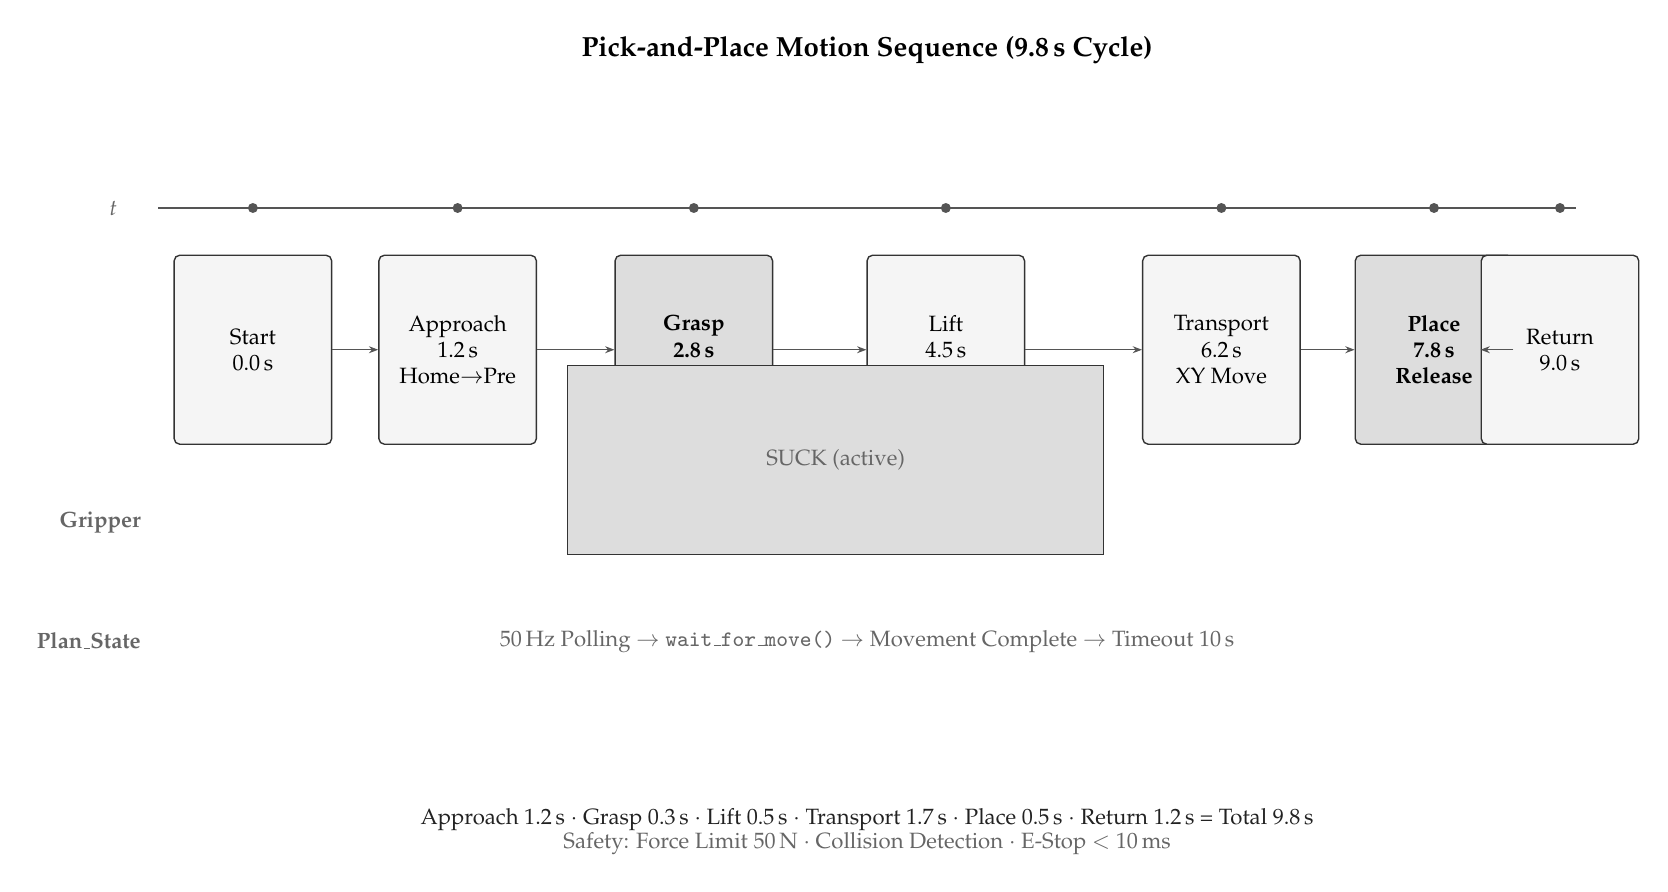
\begin{tikzpicture}[node distance=0.4cm]

  \node[font=\normalsize\bfseries] at (0, 8) {Pick-and-Place Motion Sequence (9.8\,s Cycle)};

  % Timeline
  \draw[arrowCol, line width=1pt] (-9, 6) -- (9, 6);
  \node[label, left=0.2cm] at (-9.2, 6) {$t$};

  % Phase markers
  \foreach \x/\t in {-7.8/0.0, -5.2/1.2, -2.2/2.8, 1/4.5, 4.5/6.2, 7.2/7.8, 8.8/9.0} {
    \fill[arrowCol] (\x, 6) circle (1.8pt);
  }

  % Phase boxes
  \node[mainbox, minimum width=2cm, minimum height=2.4cm] (p1) at (-7.8, 4.2) {Start\\0.0\,s};
  \node[mainbox, minimum width=2cm, minimum height=2.4cm] (p2) at (-5.2, 4.2) {Approach\\1.2\,s\\Home$\rightarrow$Pre};
  \node[darkbox, minimum width=2cm, minimum height=2.4cm] (p3) at (-2.2, 4.2) {Grasp\\2.8\,s\\Suck};
  \node[mainbox, minimum width=2cm, minimum height=2.4cm] (p4) at (1, 4.2) {Lift\\4.5\,s\\Safe Z};
  \node[mainbox, minimum width=2cm, minimum height=2.4cm] (p5) at (4.5, 4.2) {Transport\\6.2\,s\\XY Move};
  \node[darkbox, minimum width=2cm, minimum height=2.4cm] (p6) at (7.2, 4.2) {Place\\7.8\,s\\Release};
  \node[mainbox, minimum width=2cm, minimum height=2.4cm] (p7) at (8.8, 4.2) {Return\\9.0\,s};

  \draw[arrow, line width=0.4pt] (p1) -- (p2);
  \draw[arrow, line width=0.4pt] (p2) -- (p3);
  \draw[arrow, line width=0.4pt] (p3) -- (p4);
  \draw[arrow, line width=0.4pt] (p4) -- (p5);
  \draw[arrow, line width=0.4pt] (p5) -- (p6);
  \draw[arrow, line width=0.4pt] (p6) -- (p7);

  % Gripper state bar
  \node[label, left=0.1cm] at (-9, 2) {Gripper};
  \fill[fillDark, draw=border, line width=0.3pt] (-3.8, 1.6) rectangle (3, 4);
  \node[font=\footnotesize, text=textSub] at (-0.4, 2.8) {SUCK (active)};

  % Feedback
  \node[label, left=0.1cm] at (-9, 0.5) {\footnotesize Plan\_State};
  \node[font=\footnotesize, text=textSub] at (0, 0.5) {50\,Hz Polling $\rightarrow$ \texttt{wait\_for\_move()} $\rightarrow$ Movement Complete $\rightarrow$ Timeout 10\,s};

  % Metrics
  \node[font=\footnotesize, text=textCol, below=1.2cm] at (0, -0.3) {Approach 1.2\,s $\cdot$ Grasp 0.3\,s $\cdot$ Lift 0.5\,s $\cdot$ Transport 1.7\,s $\cdot$ Place 0.5\,s $\cdot$ Return 1.2\,s = Total 9.8\,s};
  \node[font=\footnotesize, text=textSub, below=0.6cm] at (0, -1.2) {Safety: Force Limit 50\,N $\cdot$ Collision Detection $\cdot$ E-Stop $<$ 10\,ms};

\end{tikzpicture}

% ── FIGURE 6: DQN Architecture ──
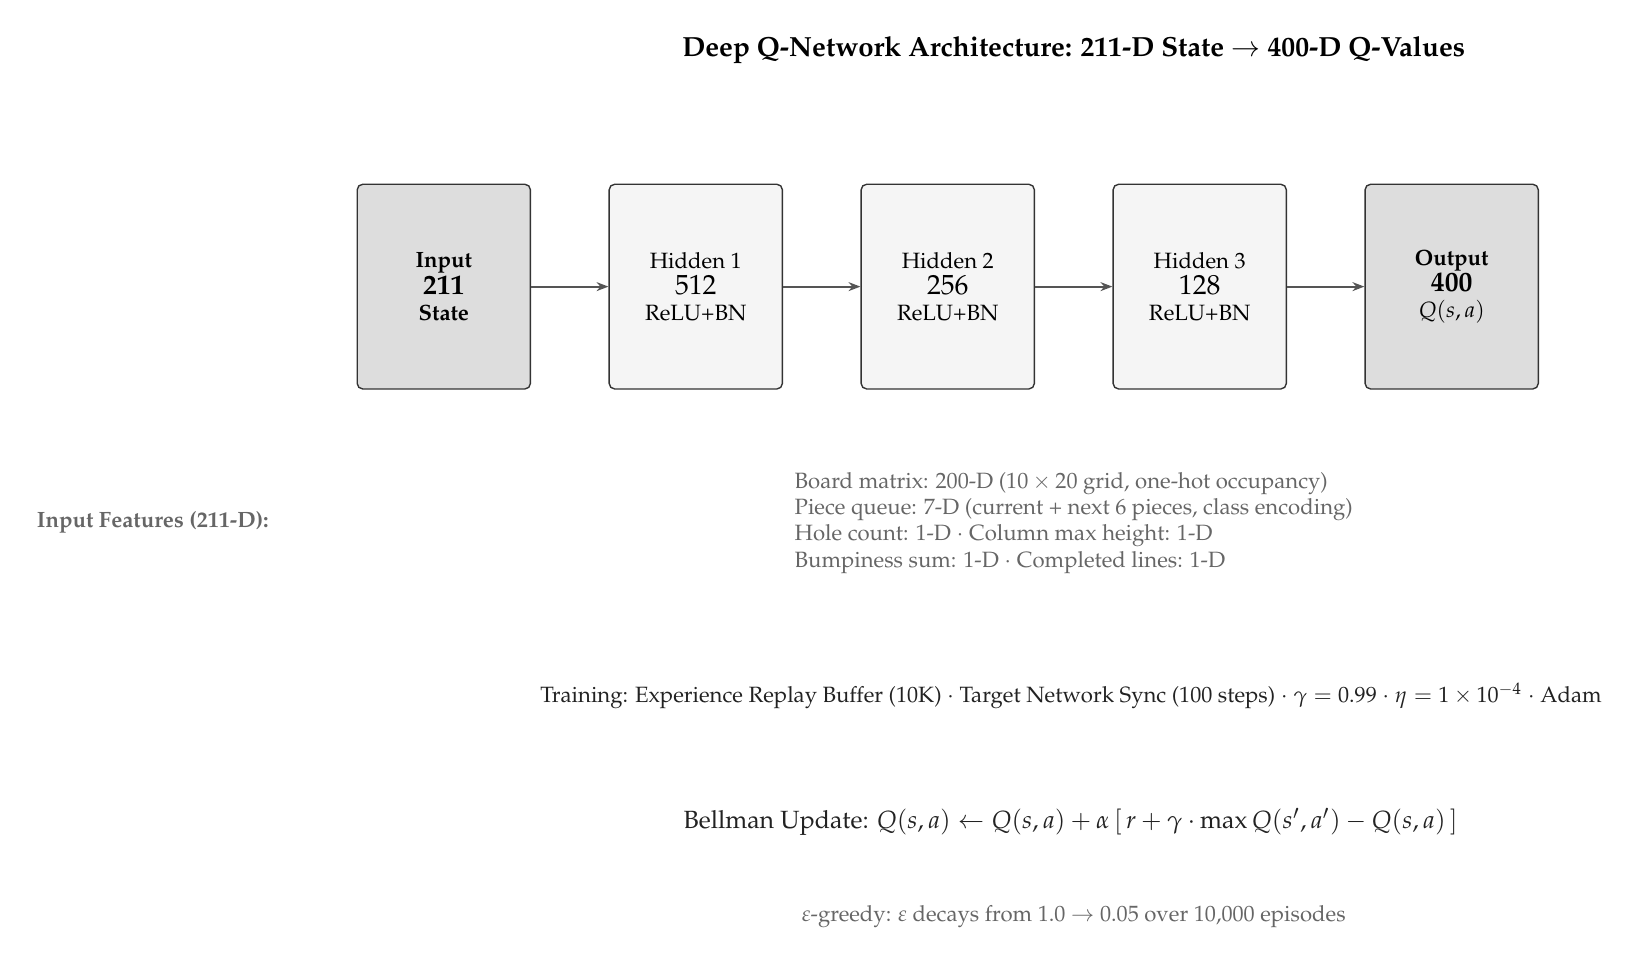
\begin{tikzpicture}[node distance=0.3cm]

  \node[font=\normalsize\bfseries] at (0, 8.5) {Deep Q-Network Architecture: 211-D State $\rightarrow$ 400-D Q-Values};

  % Layer boxes
  \node[darkbox, minimum width=2.2cm, minimum height=2.6cm] (inp) at (-8, 5.5) {Input\\\normalsize 211\\\footnotesize State};
  \node[mainbox, minimum width=2.2cm, minimum height=2.6cm] (h1) at (-4.8, 5.5) {Hidden 1\\\normalsize 512\\\footnotesize ReLU+BN};
  \node[mainbox, minimum width=2.2cm, minimum height=2.6cm] (h2) at (-1.6, 5.5) {Hidden 2\\\normalsize 256\\\footnotesize ReLU+BN};
  \node[mainbox, minimum width=2.2cm, minimum height=2.6cm] (h3) at (1.6, 5.5) {Hidden 3\\\normalsize 128\\\footnotesize ReLU+BN};
  \node[darkbox, minimum width=2.2cm, minimum height=2.6cm] (out) at (4.8, 5.5) {Output\\\normalsize 400\\\footnotesize $Q(s,a)$};

  \draw[arrow, line width=0.7pt] (inp) -- (h1);
  \draw[arrow, line width=0.7pt] (h1) -- (h2);
  \draw[arrow, line width=0.7pt] (h2) -- (h3);
  \draw[arrow, line width=0.7pt] (h3) -- (out);

  % Feature list
  \node[label, left=0.1cm] at (-10, 2.5) {\footnotesize Input Features (211-D):};
  \node[font=\footnotesize, text=textSub, align=left] at (0, 2.5) {
    Board matrix: 200-D ($10\times 20$ grid, one-hot occupancy) \\
    Piece queue: 7-D (current + next 6 pieces, class encoding) \\
    Hole count: 1-D $\cdot$ Column max height: 1-D \\
    Bumpiness sum: 1-D $\cdot$ Completed lines: 1-D
  };

  % Training
  \node[font=\footnotesize, text=textCol, align=center] at (0, 0.3) {
    Training: Experience Replay Buffer (10K) $\cdot$ Target Network Sync (100 steps) $\cdot$ $\gamma=0.99$ $\cdot$ $\eta=1\times10^{-4}$ $\cdot$ Adam
  };

  % Bellman
  \node[font=\small, text=textCol, align=center] at (0, -1.3) {
    Bellman Update: $Q(s,a) \leftarrow Q(s,a) + \alpha\,[\,r + \gamma\cdot\max Q(s',a') - Q(s,a)\,]$
  };

  \node[font=\footnotesize, text=textSub] at (0, -2.5) {$\varepsilon$-greedy: $\varepsilon$ decays from 1.0 $\rightarrow$ 0.05 over 10,000 episodes};

\end{tikzpicture}

% ── FIGURE 7: Hand-Eye Calibration ──
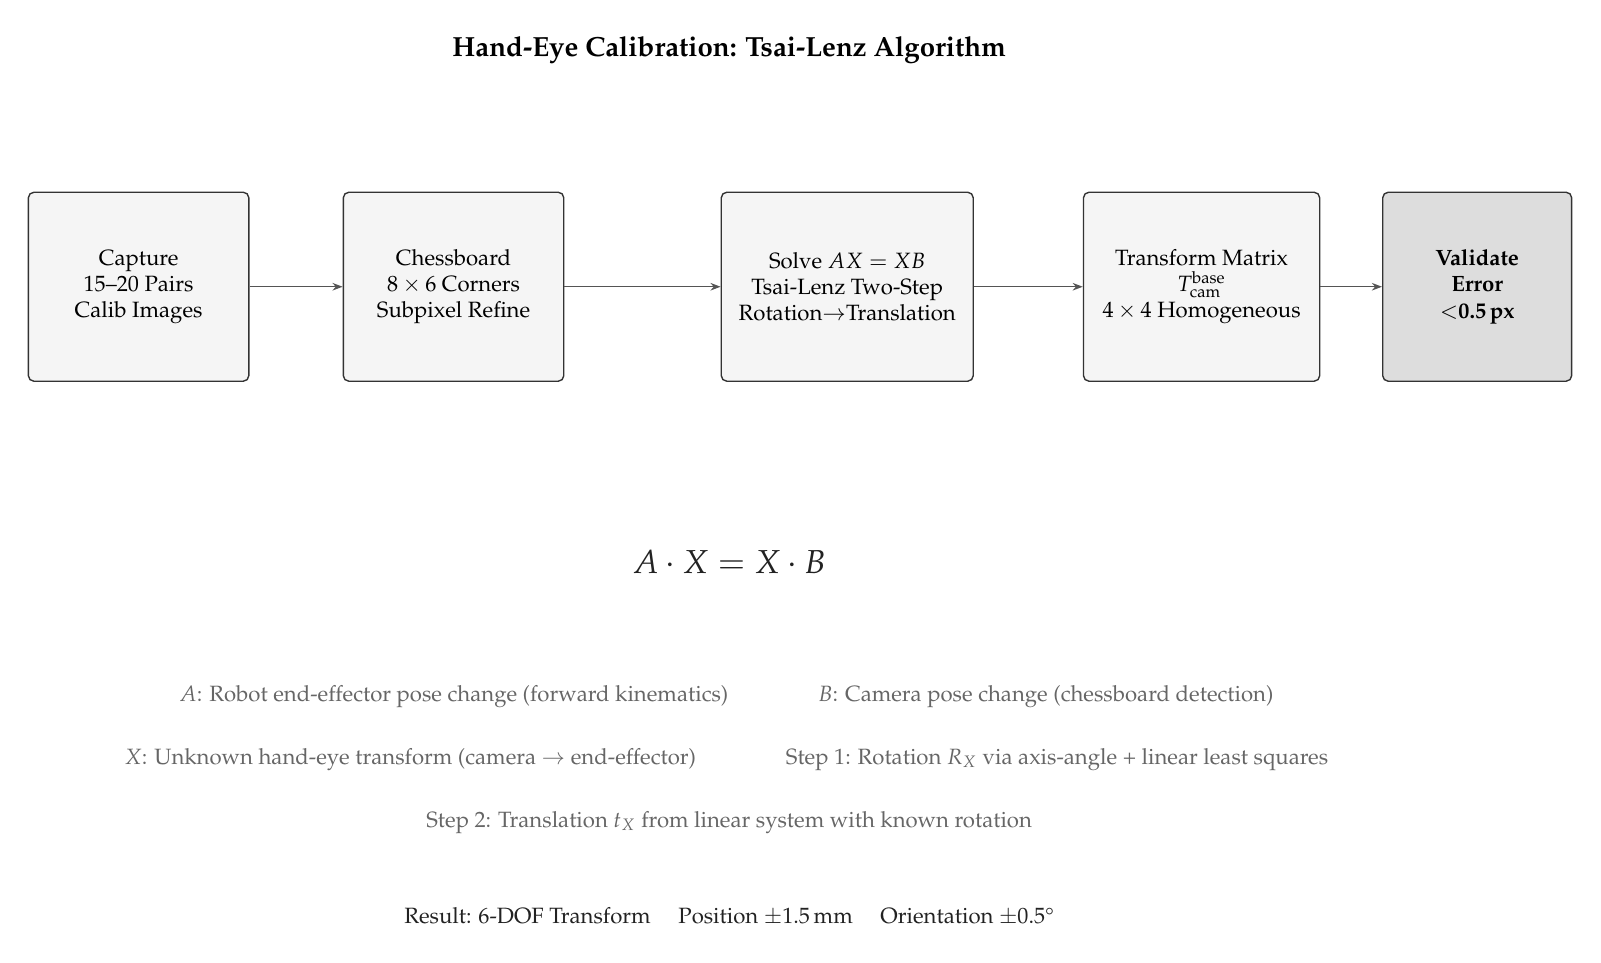
\begin{tikzpicture}[node distance=0.5cm]

  \node[font=\normalsize\bfseries] at (0, 7) {Hand-Eye Calibration: Tsai-Lenz Algorithm};

  % Steps
  \node[mainbox, minimum width=2.8cm, minimum height=2.4cm] (s1) at (-7.5, 4) {Capture\\15--20 Pairs\\Calib Images};
  \node[mainbox, minimum width=2.8cm, minimum height=2.4cm] (s2) at (-3.5, 4) {Chessboard\\$8\times 6$ Corners\\Subpixel Refine};
  \node[mainbox, minimum width=3.2cm, minimum height=2.4cm] (s3) at (1.5, 4) {Solve $AX=XB$\\Tsai-Lenz Two-Step\\Rotation$\rightarrow$Translation};
  \node[mainbox, minimum width=3cm, minimum height=2.4cm] (s4) at (6, 4) {Transform Matrix\\$T_\text{cam}^\text{base}$\\$4\times 4$ Homogeneous};
  \node[darkbox, minimum width=2.4cm, minimum height=2.4cm] (s5) at (9.5, 4) {Validate\\Error\\$<$0.5\,px};

  \draw[arrow] (s1) -- (s2);
  \draw[arrow] (s2) -- (s3);
  \draw[arrow] (s3) -- (s4);
  \draw[arrow] (s4) -- (s5);

  % AX=XB
  \node[font=\large\bfseries, text=textCol] at (0, 0.5) {$A \cdot X = X \cdot B$};

  \node[font=\footnotesize, text=textSub, align=left] at (0, -1.2) {
    $A$: Robot end-effector pose change (forward kinematics) \hspace{1cm}
    $B$: Camera pose change (chessboard detection)
  };
  \node[font=\footnotesize, text=textSub, align=left] at (0, -2) {
    $X$: Unknown hand-eye transform (camera $\rightarrow$ end-effector) \hspace{1cm}
    Step 1: Rotation $R_X$ via axis-angle + linear least squares
  };
  \node[font=\footnotesize, text=textSub] at (0, -2.8) {Step 2: Translation $t_X$ from linear system with known rotation};

  \node[font=\footnotesize, text=textCol] at (0, -4) {Result: 6-DOF Transform \quad Position $\pm$1.5\,mm \quad Orientation $\pm$0.5\textdegree};

\end{tikzpicture}

\end{document}
